\section{Quantum prototypes: changing the calculation}
\label{section:quantum-prototypes-changing-the-calculation}

The preceding examples show how representation changes the information available to a calculation. The next test is operational: can we use that information to choose better updates, trial states or measurements? We examine three operational methods: inspect feedback before its scalar projection, repair the retained trial space, and choose a spectral window whose measurements remain informative.

A pure quantum state is a vector of complex amplitudes. Their squared magnitudes give outcome probabilities in a chosen measurement basis. An observable is a Hermitian operator, and its expectation value is the average score obtained by repeatedly preparing and measuring the state. A Hamiltonian $H$ is the observable for energy. Finding its lowest-energy state is useful in molecular and materials calculations, but a general $n$-qubit state has $2^n$ amplitudes. The choice of accessible states and measurements is therefore central to the calculation.

The circuit $U$ preserves the state vector's norm. Its adjustable gates determine which states the calculation can prepare.

A variational algorithm prepares a family of states $|\psi(\theta)\rangle=U(\theta)|\psi_0\rangle$ using a parameterised circuit $U$, measures an energy or other cost, and adjusts $\theta$. It combines a quantum experiment with a classical optimiser. There are at least three different ways for this procedure to struggle. The measured scalar can conceal a useful operator change. The chosen trial family can omit the needed state. The measurement used to resolve a spectral feature can become ill-conditioned. The Eigen prototypes make those failures distinct and suggest a different repair for each.

Three operators now have distinct jobs. The differential operator $H_V$ in Eq.~\eqref{eq:loss-operator} describes relaxation of a classical density. The circuit loss operator $\mathcal L(\theta)$ describes the changing quantum observable. The Hamiltonian $H$ in the residual calculation describes the physical system whose low-energy state we seek. Spectral analysis is useful in each of these spaces.

\subsection{Operator diagnostics before scalar feedback}
The loss-operator construction starts before the scalar reading.~\cite{McCaul0c5ec5}

\begin{equation}
 {\cal L}(\theta)=U(\theta)^\dagger O U(\theta),\qquad C(\theta)=\langle\psi_0|{\cal L}(\theta)|\psi_0\rangle.
 \label{eq:operator-scalar}
\end{equation}
$O$ is the measured observable, the dagger denotes the conjugate transpose, and ${\cal L}$ retains the circuit's action on the observable. The scalar $C$ samples it with one input state. This is the familiar Heisenberg representation used for a particular purpose: distinguish information in the changing operator from the training signal exposed by one measurement functional.

At a differentiated gate, the gradient can be written as $\langle\psi|A|\psi\rangle$ for a Hermitian traceless operator $A=(i/2)[G,\Omega]$, where $G$ generates that gate, $\Omega$ is the appropriately propagated observable and $[G,\Omega]=G\Omega-\Omega G$. For a fixed $A$, if the state is drawn independently of $A$ from a state 2-design, meaning that its second moments match those of a uniformly random pure state, then
\begin{equation}
 {\rm Var}\big(\langle\psi|A|\psi\rangle\big)=\frac{{\rm Tr}(A^2)}{d(d+1)},\qquad d=2^n.
 \label{eq:operator-variance}
\end{equation}
The squared Hilbert--Schmidt norm is $\|A\|_{\rm HS}^2=\operatorname{Tr}(A^\dagger A)$. The operator can retain substantial squared norm while its scalar reading concentrates. For a Pauli observable with squared Hilbert--Schmidt norm $d$, a normalised gradient-operator fraction near one half gives variance near $1/[2(d+1)]$. The normalisation explains the scaling rather than hiding it.

The archived fixed-operator checks and two-to-eight-qubit circuit ensembles test this distinction directly. Figure~\ref{fig:dd-operator-projection} shows the scalar-gradient variance falling while the normalised operator-gradient fraction remains near one half. The local and global observable ensembles behave similarly here. The calculation explains how a substantial operator change can become difficult to see through a single scalar measurement.
\begin{figure}[htbp]
\centering
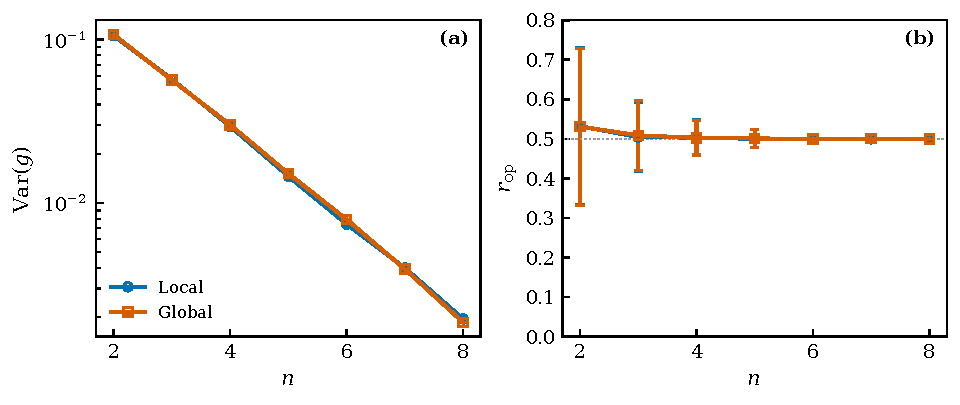
\includegraphics[width=\linewidth]{figures/portable-run-b69220b3a27348ad.result/dd-operator-projection.pdf}
\caption{Operator content and scalar feedback. Archived classical circuit-ensemble calculations, seed 20240603 and 2,000 samples per point. (a) Scalar-gradient variance $\operatorname{Var}(g)$ decreases with qubit number $n$. (b) The normalised operator-gradient fraction $r_{\rm op}=\|A\|_{\rm HS}^2/\|O\|_{\rm HS}^2$ remains near one half. Bars are archived sample standard deviations, not confidence intervals. The local and global observable ensembles nearly coincide in this experiment. The comparison isolates the scalar-projection mechanism. Measuring the operator content remains a separate resource cost.}
\label{fig:dd-operator-projection}
\end{figure}

The next design question is where that operator content sits. A Pauli string is a tensor product of the one-qubit identity and Pauli matrices $I,X,Y,Z$. For example, $X$ exchanges the two basis states and $Z$ reverses the sign of the second amplitude. Its weight counts the nonidentity factors: $Z_1X_2$, for example, has weight two. Expanding the operator in these strings groups contributions by the number of qubits on which they act. Keeping low-weight content can make measurements or local constructions manageable. The source experiments track how those bands change with circuit depth. Their useful implication is diagnostic: inspect what a scalar projection has obscured before attributing every failure to the optimiser. The tested block-and-merge training hierarchy did not outperform a deep global optimiser on the reported models up to ten qubits. The stronger practical construction comes from using a residual to change the trial representation itself.

\subsection{Residual-guided active-space repair}
The active-space repair is developed in Closure-Guided Active-Space Repair for Variational Quantum Algorithms.~\cite{McCaul8cce8c} Let $P$ be the orthogonal projector onto a retained linear state space and $Q=I-P$ onto the omitted space. Suppose the lowest eigenproblem inside $P$ has been solved, producing a normalised Ritz state $\phi$ and energy $E$:
\begin{equation}
 PHP\phi=E\phi,\qquad r=Q(H-E)\phi=QH\phi,\qquad \|r\|^2=\langle\phi|(H-E)^2|\phi\rangle.
 \label{eq:ritz-residual}
\end{equation}
The residual $r$ is the part of the full eigenvalue equation that remains unsatisfied. The internal optimiser has finished its task. Repeating that same optimisation cannot lower the minimum available inside $P$. Enlarging or rotating the retained space can.

For a normalised omitted direction $w$, write $a=\langle w|r\rangle$ and $\beta=\langle w|H|w\rangle$. Solving the two-dimensional problem on $\mathrm{span}\{\phi,w\}$ gives
\begin{equation}
 e_-=\frac{E+\beta-\sqrt{(\beta-E)^2+4|a|^2}}{2},\qquad E_{\rm enlarged}\leq e_-.
 \label{eq:ritz-descent}
\end{equation}
A nonzero overlap $a$ guarantees a strict decrease relative to $E$. The inequality matters: the whole enlarged space may do better than this two-dimensional restriction. When $\beta-E>0$ is large compared with $|a|$, the estimated gain is $|a|^2/(\beta-E)$. A larger discrepancy is not necessarily a more valuable correction if reaching it costs much more energy.

The exact block elimination behind this reasoning is the Feshbach effective operator
\begin{equation}
 H_F(E)=PHP+PHQ(E-QHQ)^{-1}QHP.
 \label{eq:feshbach}
\end{equation}
The inverse acts on the omitted space $\operatorname{Ran}(Q)$ and the expression applies where that inverse exists. In a full eigenpair, the omitted component is obtained by applying $(E-QHQ)^{-1}QHP$ to the retained component. Replacing that unknown full solution by a Ritz pair gives a practical correction approximation. The denominator supplies physical information that the raw residual alone does not contain.

The four-qubit rank-growth prototype uses
\[
 H_{\rm grow}(\lambda)=-X_0-0.7X_1+0.2Z_0Z_1
 +4(n_2+1.2n_3)+\lambda(Z_1X_2+0.7X_0X_3),
 \quad n_j=(I-Z_j)/2.
\]
Here $n_j$ penalises excitation of qubit $j$ and $\lambda$ sets the coupling to the initially omitted qubits. The initial rank-four space allows two qubits to vary and fixes the other two. At $\lambda=1$, adding two residual directions reduces the energy error by almost three orders of magnitude. A restricted pool of one- and two-qubit Pauli directions also gives a substantial improvement, and both routes reach numerical roundoff by rank ten. These exact dense-state calculations expose the effect of enlarging the representation before finite-shot measurement costs enter.

For the two-channel comparison in Figure~\ref{fig:dd-gap-selection}, the model is
\begin{align}
H(\lambda)={}&-X_0-0.7X_1+0.2Z_0Z_1+0.4n_2+30n_3\nonumber\\
 &+\lambda(0.8Z_1X_2+0.9X_0X_3),\qquad n_j=(I-Z_j)/2 .
\end{align}
The operator $n_j$ penalises excitation of qubit $j$. Initially qubits 0 and 1 vary, while qubits 2 and 3 remain in $|00\rangle$. The candidate pool contains the two displayed boundary operators. One excites a cheap omitted degree of freedom, the other an expensive one. This is a separate multiscale test from the preceding rank-growth example.

The multiscale example separates the size of a coupling from the benefit of following it. The channel with the larger raw overlap is much more expensive to excite. The smaller-overlap, low-gap direction therefore produces the larger energy decrease. Figure~\ref{fig:dd-gap-selection} compares the resulting errors across coupling strengths: denominator-aware selection spends the same extra direction where it changes the answer most.
\begin{figure}[htbp]
\centering
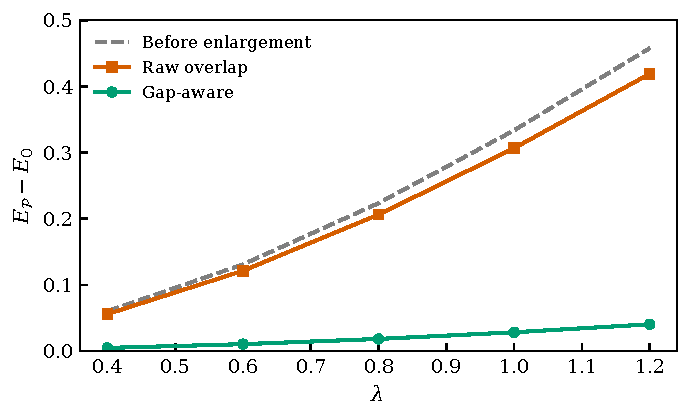
\includegraphics[width=\linewidth]{figures/portable-run-b69220b3a27348ad.result/dd-gap-selection.pdf}
\caption{Choose an omitted direction by its value, not only its amplitude. Each method adds one direction from the same pool in the archived residual prototype. Coupling $\lambda$ and retained-space energy error $E_P-E_0$ use the model's dimensionless units. Raw residual amplitude favours a high-gap channel. The implemented amplitude-over-gap rule selects a more useful low-gap channel and leaves a smaller error. The curves are exact dense-state calculations for the displayed Hamiltonian and two-candidate pool.}
\label{fig:dd-gap-selection}
\end{figure}

For normalised candidates, the implemented amplitude-over-gap score is $|a|/|\beta-E|$. The second-order energy-gain estimate is $|a|^2/(\beta-E)$ when $\beta-E>0$ is large compared with $|a|$. These are different rankings in general, although both select the useful channel here. Their distinction belongs in the reproducible algorithm specification. The relevant prior comparison is ADAPT-VQE, which already grows an ansatz by testing a pool of candidate operators. Its original ranking uses energy gradients rather than an energy denominator, and it trades a more compact circuit for extra pool measurements.\footnote{H. R. Grimsley et al., \emph{An adaptive variational algorithm for exact molecular simulations on a quantum computer}, Nature Communications 10 (2019), \href{https://doi.org/10.1038/s41467-019-10988-2}{doi:10.1038/s41467-019-10988-2}.} Eigen's residual examples motivate a testable improvement in selection, not a claim to have invented adaptive ansatz growth.~\cite{Grimsley20198f59be}

There is also a revealing success at the end of the rank-growth calculation. The target state's residual becomes negligible while the whole-space leakage $\|QHP\|$ remains finite. The desired eigenstate has been captured, but the retained space is not invariant for every state it contains. A zero residual by itself certifies an eigenpair, not the ground state: for $H=\operatorname{diag}(0,1)$ and $P$ retaining only the second coordinate, the lowest-in-$P$ pair has $E=1$ and $r=0$, while the true ground energy is zero. Ground-state certification therefore needs an additional bound or spectral condition. This is precisely the task-relative distinction introduced by the four-state process. Fidelity to the required answer can be cheaper than closure of the whole description.

\subsection{Spectral windows with reusable measurements}
Spectral estimation asks a related question about resolution rather than trial-space size. For a probe energy $\lambda$ and $\tau>0$, define
\begin{align}
 Z_\tau(\lambda)&=\langle\psi_0|e^{-\tau(H-\lambda)^2}|\psi_0\rangle,\nonumber\\
 N_\tau(\lambda)&=\langle\psi_0|H e^{-\tau(H-\lambda)^2}|\psi_0\rangle,\qquad F_\tau=\frac{N_\tau}{Z_\tau}.
 \label{eq:spectral-filter}
\end{align}
The Gaussian selects energies within a width of order $\tau^{-1/2}$ around $\lambda$. $F_\tau$ is their weighted mean. Moving the window traces supported spectral levels. An eigenvalue with zero input-state weight remains invisible to this expectation.

For a self-adjoint $H$, the exact Fourier identity
\begin{equation}
 e^{-\tau(H-\lambda)^2}=\frac{1}{\sqrt{4\pi\tau}}\int_{-\infty}^{\infty}e^{-s^2/(4\tau)}e^{-is(H-\lambda)}\,ds
 \label{eq:gaussian-fourier}
\end{equation}
expresses the filter through real-time unitary evolution. Quantum hardware naturally implements those rotations. The probe energy enters as a classical phase, so the same measured overlaps can be reweighted for several windows. Figure~\ref{fig:dd-spectral-window} explains this reuse. A narrower energy question requires longer time information and more precise estimation, not merely a different label on the plot.
\begin{figure}[htbp]
\centering
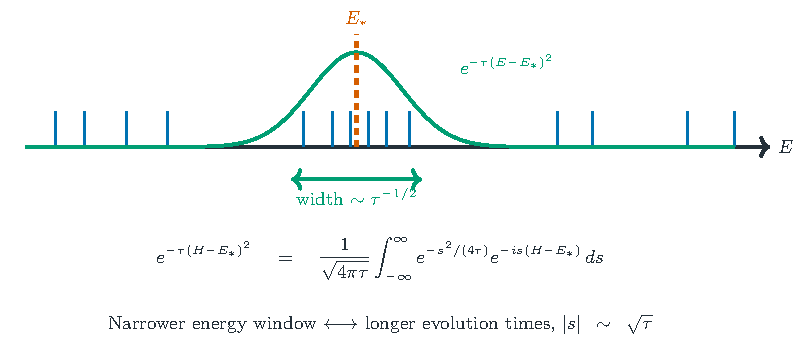
\includegraphics[width=\linewidth]{figures/portable-run-b69220b3a27348ad.result/dd-spectral-window.pdf}
\caption{A spectral window and its time-domain cost. For self-adjoint $H$, real probe energy $E_\star$ and $\tau>0$, the Gaussian width scales as $\tau^{-1/2}$. The Fourier representation uses real-time evolution on a scale proportional to $\sqrt{\tau}$, with $\hbar=1$. Here $E_\star$ is the probe denoted $\lambda$ in Eq.~\eqref{eq:spectral-filter}. Narrower resolution requires longer-time information. ITQDE supplies the overlap construction, while Free Snacks examines local support and conditioning. This is a mathematical schematic, not a measured spectrum.}
\label{fig:dd-spectral-window}
\end{figure}

Quantum Dynamical Emulation of Imaginary Time Evolution, or ITQDE, provides a concrete measurement construction. It reconstructs filtered expectations from forward/backward overlaps using ancilla-assisted tests. The paper includes a two-system-qubit IBM Brisbane experiment with 104 random Clifford initial states and 4,000 samples per overlap, alongside separate numerical and simulator examples. This is evidence that the overlap route can be implemented on hardware at that scale. Its economy is reuse and reduced coherent-circuit requirements, paid for with sampling rather than free preparation of a filtered state.~\cite{Leamer20249db941}

Free Snacks in Quantum Complexity~\cite{McCaul2025f7b569} focuses on when the ratio becomes unreliable. With estimated errors $\delta N,\delta Z$ and $|\delta Z|<Z$, elementary rearrangement gives
\[
 |\widehat F-F|\leq\frac{|\delta N|+|F|\,|\delta Z|}{Z-|\delta Z|}.
\]
A narrow window placed between widely separated supported levels has a small denominator. Even accurate overlap estimates can then give an unstable ratio. Within the paper's additive-noise model, resolving a very small gap while crossing a large one can demand a rapidly growing sample budget. The relevant bandwidth is a ratio of scales in the chosen spectral window, not simply the total number of qubits.

Local coarsening offers a controlled response. Convolving the numerator and denominator separately in probe energy with a normalised Gaussian of variance $\sigma^2$ gives a common prefactor $(1+2\tau\sigma^2)^{-1/2}$ and replaces $\tau$ by $\tau/(1+2\tau\sigma^2)$. The prefactor cancels in their ratio. This square-completion calculation uses separate numerator and denominator smoothing, which is generally different from smoothing their ratio. Existing overlap data can therefore answer a coarser question without rerunning a separate circuit for every probe energy. The price is merging distinctions. Whether that is acceptable depends on the observable or decision being sought.

Together, these prototypes supply a practical programme. Preserve the operator information that a scalar reading hides. Add omitted directions according to their expected value, not merely their magnitude. Choose spectral resolution where the estimator can support it. Candidate preparation, measurements, optimisation and conditioning then belong in one cost comparison. The same design problem appears when the large object is a collection of records rather than a quantum state: retain what a future query will need, and provide a way to recover what the smaller description omits.

